\chapter{Physical Design}
The trends nowadays is to build more complex system (in terms of transistors) in less time (reduce the time-to-market), so we need some powerful tools that allows us to have optimized ICs. The design flow strategy is based on multi-abstraction 3-step iteration; essentially the each
abstract we must do 3-steps:
\begin{enumerate}
	\item The hardware is described using a Hardware Description Language, as VHDL
	\item The Synthesis phase takes as input the abstract model and generates a more detailed model that contains additional informational information about timing, power consumption and area. The next step is the Optimization, that is used in order to generate a behaviour equivalent circuit and at the same time satisfy some conditions, like timing
	\item A post synthesis simulation is run to check the functional properties of the final model
\end{enumerate}
\section{Synthesis}
\label{sec:syn_opt}
The Synthesis has been done with an intensive script usage; in fact, two scripts have been developed in order to setup the environment, perform the synthesis and clean-up all the temporary useless files generated during the process.\newline\newline
The first script, is a bash script (refer to Appendix \ref{bash_syn}) and, as anticipated before, it is used to setup the environment by coping the \texttt{.synopsys\_dc.setup} file, copy the library and call the synthesis script suing \texttt{dc\_shell}.
Once the synthesis has been ended, the bash scripts removes all temporary folders like \texttt{ARCH}, \texttt{DOBY} and so on and moves the synthesized DLX, in both verilog and VHDL, and the all the generated reports into a specific folder.\newline\newline

The second script, that is run under the \texttt{dc\_shell} to perform the actual synthesis, performs multiple steps (refer to Appendix \ref{tcl_syn}):
\begin{itemize}
	\itemsep0sp
	\item Analyze all the .vhd files needed for the DLX
	\item Elaborate the DLX design, by correctly configuring the generics
	\item Set the wire model and create a clock, that is the constraint
	\item Perform the compilation
	\item Save the synthesized DLX
	\item Save the timing, area and power report 
\end{itemize}
The clock timing, that has been set to 2.5, has been selected after many trials and errors, in order to find the lowest possible value. Critical paths, like the one that uses the adder has been reduced using a mode optimized solution, e.g. P4 adder.\newline\newline
All complete reports are reported at Appendix \ref{ap3}; from the area report it's possible to observe that the total cell area is 35278.25 that is divided into 19747.84 for the combinational part and 15530.41 for the non combination one.\newline\newline
Another important information, that can be extracted from the timing report is, given a timing constraint, the \textit{slack}. It represents the time margin that the worst path has; in this way, the clock in the synthesis script can be tuned in order to reduce it as much as possible to increase the performances.

\section{Place and Route}
The Placement step consists on placing all the block and I/O pins within a defined area that is the chip. After this macro-step and all the units are placed, the routing is performed in order to connect all block together. After the place and route are both completed, a simulation ensures that the everything is correct. The final result can be observed at Figure \ref{fig:phy_end}.


\begin{figure}[h!]
	\begin{subfigure}[t]{.45\textwidth}
		\centering
		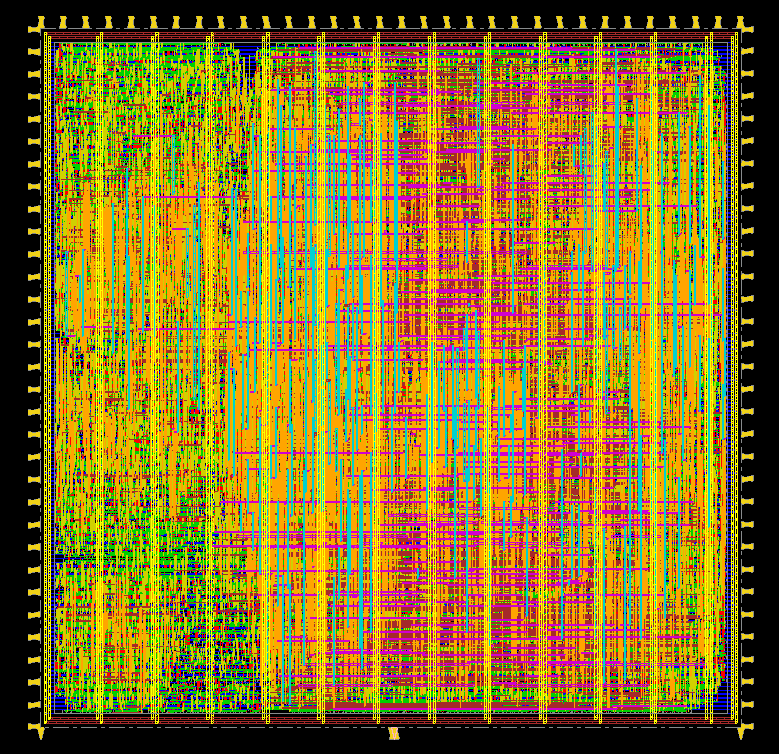
\includegraphics[width=.9\textwidth]{chapters/9_PhysicalDesign/images/pre_routing.png}
		\caption{DLX processor before routing, only logical connections are present}
		\label{fig:pre_routing}
	\end{subfigure}\hfill
	\begin{subfigure}[t]{.45\textwidth}
		\centering
		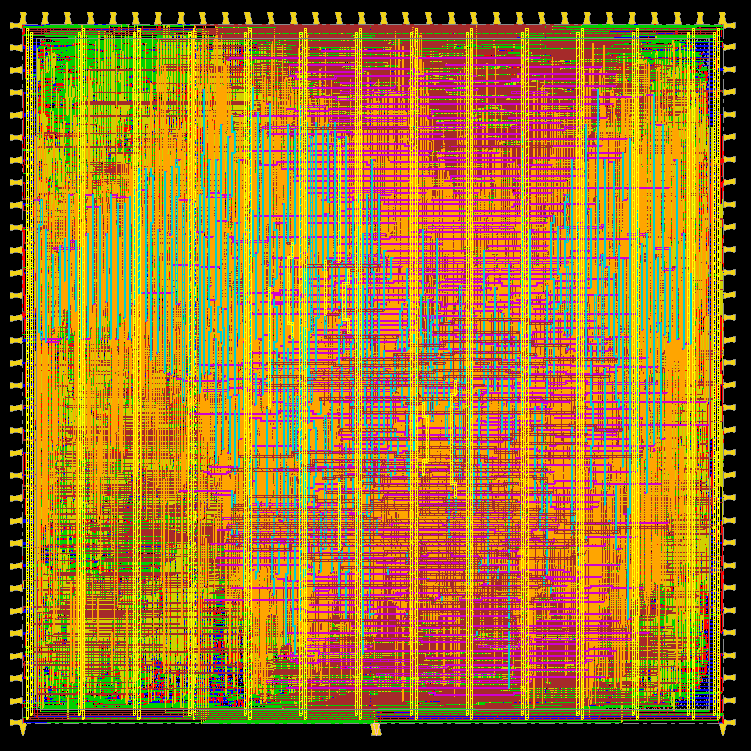
\includegraphics[width=.9\textwidth]{chapters/9_PhysicalDesign/images/phy_end.png}
		\caption{DLX processor after Place and Route phases}
		\label{fig:phy_end}
	\end{subfigure}
	\caption{DLX Place and Route}
\end{figure}

In order to obtain a fully placed and routed DLX, many steps are performed:
\begin{itemize}
	\item Structuring the Floorplan: in this step, after the Verilog file has been loaded using a global file called \texttt{DLX.globals}, a specif amount of area is dedicated to the core, while the external one is used for the power rings;
	\item Power distribution: around the core, two metal rings are positioned for distributing the power supply, so both GND and $V_{dd}$. This is not enough, since the power and ground signals must be correctly distributed. For this reason, multiple vertical metal wires, called strips, are added to the physical layout. A trade off between the number of stripes must be found, since an high number of them could lead to some problems during the cells routing. Moreover, horizontal wires are placed to prepare $V_{dd}$ and GND for the standard cells. The results is visible at Figure \ref{stripes};
	\begin{figure}[h]   
		\centering
		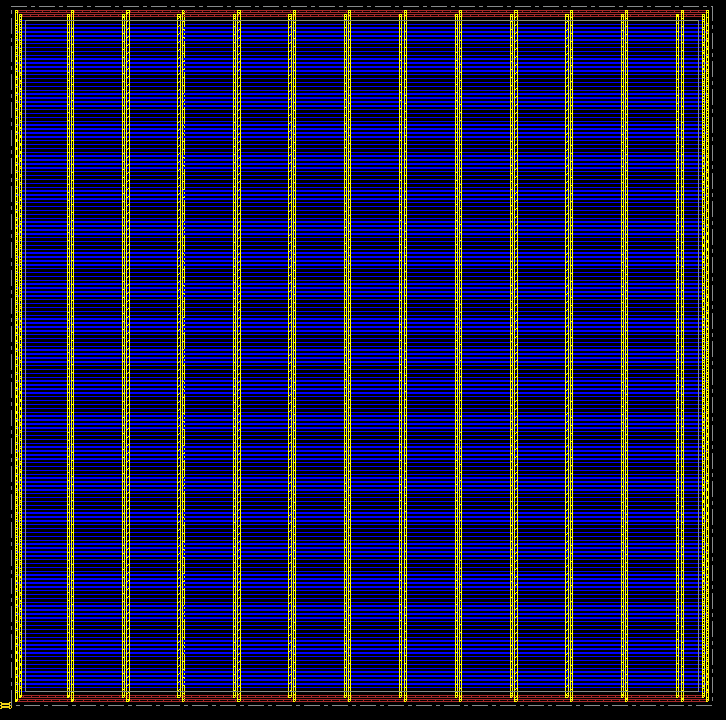
\includegraphics[width=0.38\textwidth]{chapters/9_PhysicalDesign/images/pwr_distribution.png}
		\caption{Result after placing GND and $V_{dd}$ rings with vertical and horizontal stripes.}
		\label{stripes}
	\end{figure}
	
	\item I/O placing: at this point, cells and I/O pins can be placed. Before filling the empty spaces with filler cells a Post Clock-Tree-Synthesis (CTS) optimization is performed. The result is visible at Figure \ref{fig:pre_routing};
	\item Routing: the last step is the routing, logical interconnections are replaced with physical interconnections between cells, considering the available stripes and metal rings. The design is now completed but a post routing optimization has been performed in order to respect the required timing constraints.
	

	 
\end{itemize}
